\documentclass{beamer}
\usepackage{hyperref}
\usepackage[czech]{babel}

%\usetheme{Boadilla}
\usetheme{default}
\usecolortheme{seahorse}
\definecolor{myblue}{rgb}{0.2, 0.2, 0.6}
\setbeamertemplate{caption}{{\color{myblue}Obrázek:} \raggedright\insertcaption\par}
\setbeamertemplate{footline}[frame number] 

\newcommand{\authorname}{Dluhoš Matěj, Gaja Jan, Gajdošík Petr, Jurásek Petr, Phan Thanh Tú, Rádl Jan}
\newcommand{\authorsshort}{Dluhoš, Gaja, Gajdošík, Jurásek, Phan, Rádl}
\newcommand{\thesisname}{PDS: Python}

\title{\thesisname}
\author{\authorname}
\institute{Univerzita Palackého v Olomouci}
\date{\today}

\setbeamertemplate{navigation symbols}{}
\setbeamertemplate{headline}{}
\setbeamertemplate{footline}{
  \leavevmode%
  \hbox{%
  \begin{beamercolorbox}[wd=.4\paperwidth,ht=2.25ex,dp=1ex,center]{author in head/foot}%
    \usebeamerfont{author in head/foot}\authorsshort
  \end{beamercolorbox}%
  \begin{beamercolorbox}[wd=.3\paperwidth,ht=2.25ex,dp=1ex,center]{title in head/foot}%
    \usebeamerfont{title in head/foot}\thesisname
  \end{beamercolorbox}%
  \begin{beamercolorbox}[wd=.3\paperwidth,ht=2.25ex,dp=1ex,right]{date in head/foot}%
    \usebeamerfont{date in head/foot}\insertshortdate{}\hspace*{2em}
    \insertframenumber{} / \inserttotalframenumber\hspace*{2ex} 
  \end{beamercolorbox}}%
  \vskip0pt%
}

%\logo{\includegraphics[height=1cm]{UP_logo.png}}
\usepackage{tikz}
\addtobeamertemplate{headline}{}{%
    \begin{tikzpicture}[overlay, remember picture]
    	\ifnum\insertframenumber>1
        	\node[anchor=north east, inner sep=5pt] at (current page.north east) {\includegraphics[height=1cm]{obrazky/UP_logo.png}};
        \fi
    \end{tikzpicture}
}

\setbeamercolor{titlelike}{bg=,fg=}

\begin{document}

\begin{frame}
	\titlepage
\end{frame}

\begin{frame}{Obsah}
	\tableofcontents
\end{frame}

\section{Úvod do Pythonu s paralelismem}
\subsection{Historie a zaměření}
\begin{frame}{Historie a zaměření}
    \begin{columns}
        \column{0.55\textwidth}
        \begin{itemize}
            \item Vytvořen \textbf{Guidem van Rossumem} v roce \textbf{1991}.
            \item Jednoduchost a čitelnost kódu.
            \item Vysoká produktivita programátorů.
            \item Univerzální použití: od webových aplikací přes vědecké výpočty až po strojové učení.
            \item Python získal základní podporu paralelismu prostřednictvím vláken ve verzi 1.5.2 (1999).
        \end{itemize}
        
        \column{0.45\textwidth}
        \begin{figure}
        		\includegraphics[width=0.75\textwidth]{obrazky/Guido_van_Rossum.jpg}
        		\caption{Guido van Rossum}
      		\end{figure}
    \end{columns}
\end{frame}

\subsection{GIL - Global Interpreter Lock}
\begin{frame}{Co to je GIL a proč je potřeba?}
	\textbf{Co to je GIL?}
	\begin{itemize}
		\item GIL je mutex umožňující pouze jednomu vláknu mít kontrolu nad Python interpreterem.
	\end{itemize}
	\textbf{Proč je potřeba?}
	\begin{itemize}
		\item Správa paměti v CPythonu není bezpečná pro více vláken.
		\item Python využívá počítání referencí.
		\item Problém nastane, když dvě vlákna současně zvyšují nebo snižují referenci.
		\item To vede k úniku nebo k nesprávnému uvolnění paměti.
	\end{itemize}
\end{frame}

\subsection{Rozdíl vláken a procesů}
\begin{frame}{Vlákno}
	\begin{itemize}
		\item Entita v rámci procesu.
		\item \textbf{Klíčová fakta:}
			\begin{itemize}
				\item [\textendash] V rámci jednoho procesu může být spuštěno více vláken.
				\item [\textendash] Paměť je sdílena mezi všemi vlákny.
				\item [\textendash] Spuštění vlákna je rychlejší než spuštění procesu.
				\item [\textendash] Skvělé pro úlohy závislé na I/O.
				\item [\textendash] Lehká paměťová náročnost.
			\end{itemize}
		\item \textbf{Nevýhody:}
			\begin{itemize}
				\item [\textendash] Jedno GIL pro všechna vlákna.
				\item [\textendash] Multithreading nemá efekt u úloh náročných na CPU.
				\item [\textendash] Vlákna nelze přerušit a ukončit.
				\item [\textendash] Zvýšený potenciál vzniku chyby souběhu.
			\end{itemize}
	\end{itemize}
\end{frame}

\begin{frame}{Proces}
	\begin{itemize}
		\item Instance programu.
		\item \textbf{Klíčová fakta:}
			\begin{itemize}
				\item [\textendash] Využívá více jader a procesorů.
				\item [\textendash] Nový proces se spouští nezávisle na prvním procesu.
				\item [\textendash] Má oddělený paměťový prostor.
				\item [\textendash] Každý proces má svůj vlastní GIL.
				\item [\textendash] Ideální pro úlohy náročné na CPU.
				\item [\textendash] Procesy lze přerušit nebo ukončit.
			\end{itemize}
		\item \textbf{Nevýhody:}
			\begin{itemize}
				\item [\textendash] Spuštění procesu je pomalejší než spuštění vlákna.
				\item [\textendash] Vyšší paměťová náročnost.
				\item [\textendash] Složitější IPC.
			\end{itemize}
	\end{itemize}
\end{frame}

\begin{frame}{Potřebujeme vůbec GIL?}
	\textbf{Je tedy potřeba?}
	\begin{itemize}
		\item V brzkých dnech Pythonu usnadnil integraci nativního kódu v C.
		\item Vyřešil problémy s přístupem ke sdíleným datům.
		\item Optimalizoval výkon na systémech s jedním jádrem.
	\end{itemize}
	\textbf{Ale...}
	\begin{itemize}
		\item Omezuje paralelní výkon na vícejádrových procesorech.
		\item Vede k neefektivnímu využití vláken u CPU-bound úloh.
	\end{itemize}
	\textbf{\hypersetup{urlcolor=blue} \href{https://peps.python.org/pep-0703/}{PEP 703}} - Making the Global Interpreter Lock Optional in CPython.
\end{frame}


%\subsection{Paralelismus v Pythonu}
%\begin{frame}{Paralelismus v Pythonu}
%	\begin{itemize}
%		\item Python získal základní podporu paralelismu prostřednictvím vláken ve verzi 1.5.2 (1999).
%		\item Zaveden \textbf{GIL} (Global Interpreter Lock)
%		\begin{itemize}
%			\item [\textendash] Usnadnilo integraci nativního kódu v C.
%			\item [\textendash] Vyřešilo problémy s přístupem ke sdíleným datům ve více vláknech.
%			\item [\textendash] Optimalizovalo výkon na systémech s jedním jádrem.
%			\item [\textendash] Omezuje paralelní výkon na vícejádrových procesorech.
%			\item [\textendash] Vede k neefektivnímu využití vláken u \textbf{CPU-bound} úloh.
%			\item [\textendash] \hypersetup{urlcolor=blue} \href{https://peps.python.org/pep-0703/}{PEP 703} - Making the Global Interpreter Lock Optional in CPython 
%		\end{itemize}
%	\end{itemize}
%\end{frame}

%\subsection{Proč odstranit GIL?}
%\begin{frame}{Proč odstranit GIL?}
%	\begin{itemize}
%		\item Většina zařízení dnes obsahuje vícejádrové procesory, kde GIL představuje významné omezení.
%		\item Efektivnější paralelní výpočty, například v oblastech umělé inteligence nebo numerických simulacích.
%		\item Výzvy při odstranění GIL:
%		\begin{itemize}
%			\item [\textendash] Potřeba bezpečného a efektivního spravování sdílené paměti (například více zamykání nebo jiných synchronizačních mechanismů).
%			\item [\textendash] Zvýšení složitosti implementace interpretu Pythonu.
%		\end{itemize}
%	\end{itemize}
%\end{frame}


\section{Synchronizační nástroje standardní knihovny}
\subsection{Knihovna threading}

\begin{frame}{Knihovna threading}
    \begin{itemize}
        \item Vestavený modul pro paralelní spouštění vláken
        \item Omezena GIL
        \item Vlákna využívají stejný paměťový prostor
        \vskip 0.35in
        \item Často využíváné pro:
        \begin{itemize}
            \item I/O operace (Read/Write, Síťování, user input)
            \item Grafické uživatelské rozhraní 
        \end{itemize}
    \end{itemize}
\end{frame}

\begin{frame}[fragile]{Třída Thread}
    \begin{itemize}
        \item Instance reprezentuje vlákno
        \item Předání funkce a argumentů
        \vskip 0.2in

        \item \textit{start()} - spustí vytvořené vlákno
        \item \textit{join()} – Počká na dokončení práce vlákna
        \item \textit{is\_alive()} – Pracuje stále vlákno?
        \item \textit{local()} – data konkrétního vlákna

        \vskip 0.2in
        \item Při práci s vlákny může dojít k synchronizačním problémům
        \item Modul poskytuje mnoho synchronizačních nástrojů
    \end{itemize}
    \scriptsize

    % t = threading.Thread(target=some_function, args=(some_arg,))
    % t.start()
    % # Nějaký kód
    % t.join()
    \begin{center}
        
\includegraphics[width=\textwidth]{obrazky/codes/carbon1.png}
    \end{center}
\end{frame}

\begin{frame}[fragile]{Lock}
    \begin{itemize}
            \item Zajistí, že ke sdíleným zdrojům bude mít přítup pouze jedno vlákno
            \item Můžeme zamknou příkaz nebo skupinu příkazu

            \vskip 0.15in
            \item \textit{acquire()} – zamkne objekt
            \item \textit{release()} – odemkne objekt
            \item klíčové slovo with - zamkne/odemkne blok automaticky

            \vskip 0.15in
            \item Varianta \textbf{RLock} pro rekurzivní funkce
    \end{itemize}
    \scriptsize

    % lock = threading.Lock()
    %
    % def function():
	%     # Nějaký kód
	%     with lock:  
	%         # Další kód
    \begin{center}
        
\includegraphics[width=\textwidth]{obrazky/codes/carbon2.png}
    \end{center}
\end{frame}

\begin{frame}[fragile]{Semaphore}
    \begin{itemize}
        \item Dokáže omezit počet vláken, které mají přístup ke zdroji
        \item Konstruktor očekává value, určuje maximální počet přístupů ke zdroji
        \newline (Varianta Binary Semaphore – maximálně 1 přístup)

        \vskip 0.25in
        \item \textit{acquire()} – zjistí jestli je count $>$ 0, pokud ano, dekrementuje count, jinak zablokuje vlákno
        \item \textit{release()} – inkrementuje count, umožní tak dalšímu vláknu přístup
        \item Opět with statement dělá automaticky
    \end{itemize}
    \scriptsize
    % sem = threading.Semaphore(limit)
    %
    % def function():
    %    # Nějaký kód
    %    with sem:
    %        # kritická sekce
    \begin{center}
        
\includegraphics[width=\textwidth]{obrazky/codes/carbon3.png}
    \end{center}
\end{frame}

\begin{frame}[fragile]{Barrier}
    \begin{itemize}
        \item Umožňuje zablokovat vlákna, dokud všechna nedojdou na určité místo v programu
        \item Až všechna vlákna dosáhnou bariéry, pokračují dál v práci
        \item Vhodné pokud vlákna pracují ve fázích, kdy po dokončení jedné se spustí další

        \vskip 0.25in
        \item \textit{wait()} – Místo, kde se vlákno zastaví, dokud ostatní vlákna k němu nedojdou
    \end{itemize}
    \scriptsize

    % barrier = threading.Barrier(limit)
    %
    % def function():
    %     # Nějaký kód
    %     barrier.wait()
    %     # Další kód
    \begin{center}
        
\includegraphics[width=\textwidth]{obrazky/codes/carbon4.png}
    \end{center}
\end{frame}

\begin{frame}{Event}
    \begin{itemize}
        \item Jednoduchý mechanizmus, který umožňuje signalizaci mezi vlákny
        \item Používá interní příznak, který nabývá hodnoty True nebo False
        \vskip 0.25in

        \item \textit{wait()} – vlákna budou blokována, dokud nebude flag nastaven na True
        \item \textit{set()} – Nastaví flag na True, vlákna volající wait() budou propuštěna
        \item \textit{clear()} – Nastaví flag na False, vlákna volající wait() budou zablokována
    \end{itemize}
\end{frame}

\begin{frame}[fragile]{Event}
    % event = threading.Event()
    %
    % def function1():
    % 	# Nějaký kód
    % 	event.wait()
    % 	# Další kód
    %
    % def function2():
    % 	# Nějaký kód
    % 	event.set()
    % 	# Další kód
    \begin{center}
        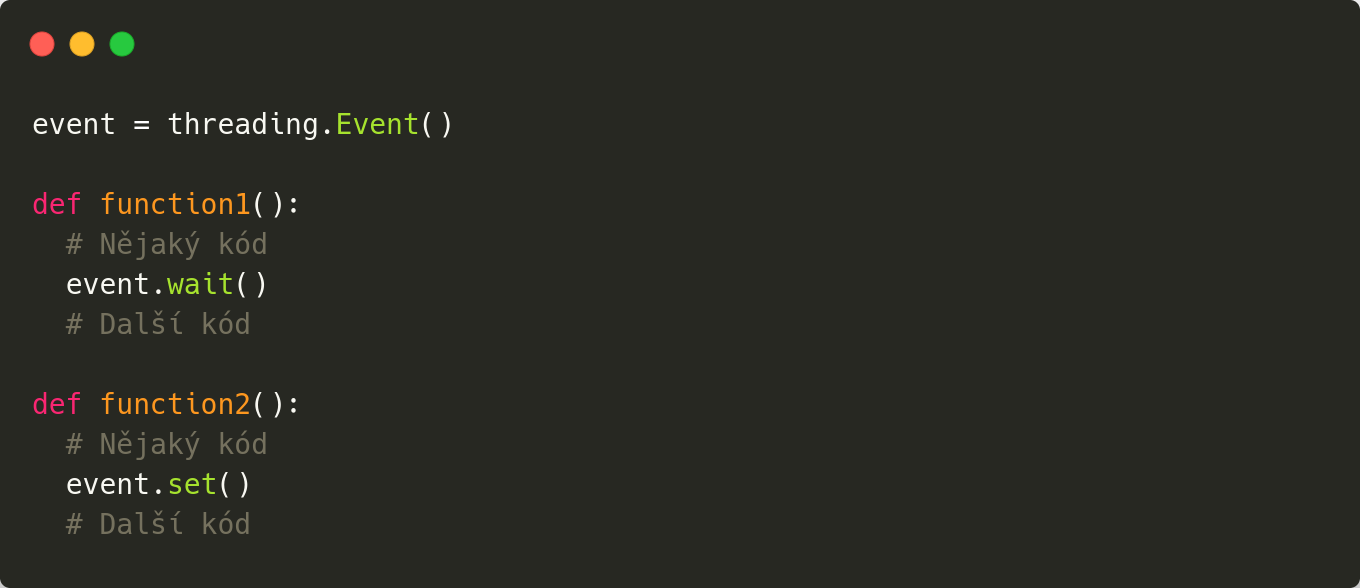
\includegraphics[width=\textwidth]{obrazky/codes/carbon5.png}
    \end{center}
\end{frame}

\begin{frame}[fragile]{Condition}
    \begin{itemize}
        \item Funguje obdobně, ale používá se současně se zámkem

        \vskip 0.25in
        \item \textit{wait()} – stejné, ale navíc odemkne zámek
        \item \textit{notify()} – odblokuje jedno čekající vlákno
        \item \textit{notify\_all()} – odblokuje všechna čekající vlákna
    \end{itemize}
    \scriptsize

    % cond = threading.Condition()
    %
    % def function1():
    % 	with cond:
    % 		# Nějaký kód
    % 		cond.wait()
    % 		# Další kód
    % 
    % def function2():
    % 	with cond:
    % 		# Nějaký kód
    % 		cond.notify()
    % 		# Další kód
    \begin{center}
        
\includegraphics[width=\textwidth]{obrazky/codes/carbon6.png}
    \end{center}
\end{frame}

\subsection{Knihovna multiprocessing}
\begin{frame}{Knihovna multiprocessing}
    \begin{itemize}
        \item Modul pro paralelizaci procesů
        \item Nepracuje s vlákny ale s procesy
        \item Umožňuje překonat limitace GIL
        \item Vhodné pro složitější výpočty
        
        \vskip 0.3in
        \item Výhody:
        \begin{itemize}
            \item Každý vytvořený proces běží nezávisle a může být vykonáván na jiných jádrech procesoru
            \item Všechny procesy mají vlastní paměť
            \item Vestavené metody pro bezpečnou práci se sdílenými prostředky
        \end{itemize}
    \end{itemize}
\end{frame}

\begin{frame}[fragile]{Třída Proces}
    \begin{itemize}
        \item Instance reprezentuje jeden nezávislý proces
        \item Tvorba stejná jako u threading
        \item Stejné funkce
        \vskip 0.25in

        \item Využití Pool
        \begin{itemize}
            \item Umožňuje efektivně spravovat procesy
            \item Automatizuje jejich tvorbu a rozdělení mezi jádra CPU
            \item \textit{map()} - pro paralelní provedení funkce na každý prvek z kolekce dat
        \end{itemize}
    \end{itemize}
    \scriptsize

    % pool = Pool(processes=num_of_processes) 
    % result = pool.map(some_function, iterable_data)
    \begin{center}
        
\includegraphics[width=\textwidth]{obrazky/codes/carbon7.png}
    \end{center}
\end{frame}

\begin{frame}{Data a komunikace}
    \begin{itemize}
        \item Sdílení dat
        \begin{itemize}
            \item Modul poskytuje objekty Array a Value pro sdílení dat mezi procesy
        \end{itemize}

        \item Komunikace
        \begin{itemize}
            \item Pro plné využití síly procesů je potřeba komunikace mezi nimi
            \item Objekty Queue a Pipe pro zasílání zpráv
            \item S Queue se pracuje stejně jako s klasickou frontou
            \item Pipe je vhodnější pro komunikaci mezi pouze dvěma procesy
        \end{itemize}
        \item Synchronizace
        \begin{itemize}
            \item Stejné nástroje pro synchronizaci jako v modulu threading
            \item Lock, Semaphore, Barrier, Event, Condition
        \end{itemize}
    \end{itemize}
\end{frame}

\begin{frame}[fragile]{Data a komunikace}
    \scriptsize
    % value = Value('i', init_value)  
    % result = Array('i', size)
    % 
    % def example_function(data,value,result):  
    %     for i, num in range(5):  
    %         result[i] = num * num  
    %         value.value += num
    % 
    % q = multiprocessing.Queue()
    % conn1, conn2 = multiprocessing.Pipe()
    % 
    % def producer(conn,q):
    %     q.put("Queue Message")
    %     conn.send("Pipe Message")
    %     conn.close()
    % 
    % def consumer(conn,q):
    %     msg = q.get()
    %     print(msg)
    %     msg = conn.recv()
    %     print(msg)
    %     conn.close()
    \begin{center}
        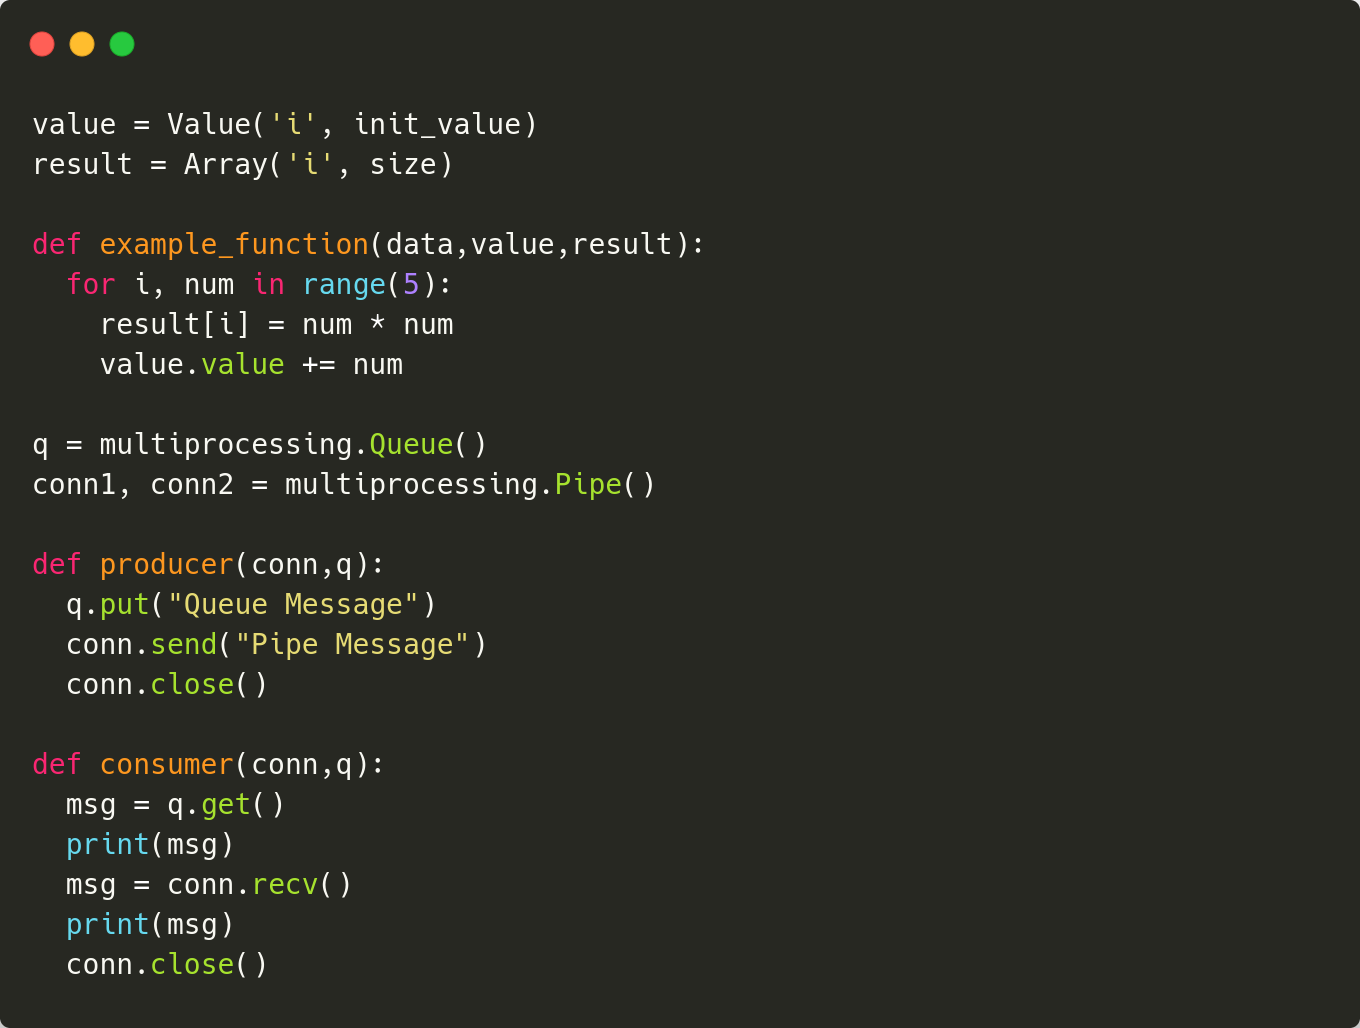
\includegraphics[width=\textwidth]{obrazky/codes/carbon8.png}
    \end{center}
\end{frame}

\subsection{Knihovna asyncio}
\begin{frame}{Knihovna asyncio}
    \begin{itemize}
        \item Umožňuje asynchronní zpracování vstupně-výstupních operací
        \item Založeno na kooperativním multitaskingu
        \item Můžeme se tak vyhnout nečinnosti při čekání na dokončení I/O operací
        \item Vhodné pro síťové operace, práce s databází, čtení souborů…
        
        \vskip 0.35in
        \item \textbf{Event Loop} – koordinuje spuštění asynchronních operací
        \item \textbf{Coroutine} – speciální asynchronní funkce
        \item \textbf{Task} – zajišťuje běh coroutine v event loopu
        \item \textbf{Future} – Předběžný výsledek operace, která nebyla ještě dokončena
    \end{itemize}
\end{frame}

\begin{frame}{Třída Task}
    \begin{itemize}
        \item Při vytváření Tasku předáváme korutinu
        \item Následně je její běh naplánován Event Loopem
        \item Metody pro práci s Tasky během toho co se vykonávají
        \begin{itemize}
            \item \textit{.result()}
            \item \textit{.exception()}
            \item \textit{.cancel()}
        \end{itemize}
        
        \vskip 0.25in
        \item Další užitečné nástroje
        \begin{itemize}
            \item Stejné synchronizační nástroje jako v předchozích modulech

            \item \textit{.wait\_for()} umožňuje nastavit maximální čas čekání na dokončení. Vyvolává TimeoutError
        \end{itemize}
    \end{itemize}
\end{frame}

\begin{frame}[fragile]{Třída Task}
    \scriptsize
    % async def coroutine(): 
    % 	do_something()
    % 	# Simulace nějaké I/O operace, na kterou je potřeba počkat
    % 	await asyncio.sleep(1) 
    % 
    % async def main():
    %     task = asyncio.create_task(coroutine(arg))
    %     await task
    % 
    % asyncio.run(main())
    \begin{center}
        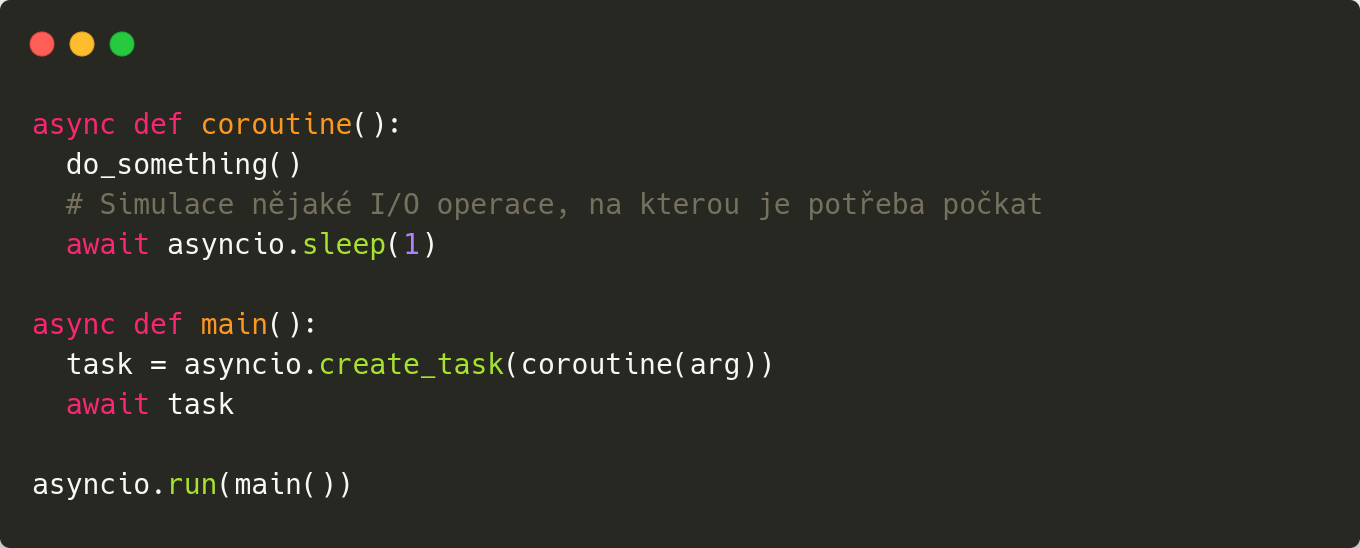
\includegraphics[width=\textwidth]{obrazky/codes/carbon9.png}
    \end{center}
\end{frame}


\section{Poznámka k paralelizaci a výkonnosti v Pythonu}
\begin{frame}{Poznámka k paralelizaci a výkonnosti v Pythonu}
	\begin{itemize}
    \item Nejde jazyk Python naproti samotné podstatě paralelizace?
    \begin{itemize}
      \item [\textendash] Známý pro svou nevýkonnost (daň za velkou abstrakci)      
      \item [\textendash] GIL
    \end{itemize}

    \item I přes omezení GIL má paralelizace opodstatnění, pokud musí vlákna často čekat na externí události (I/O)
    \begin{itemize}
      \item [\textendash] obsluha webových klientů, databáze...
      \item [\textendash] framework \textbf{asyncio} (asynchronní programování)
    \end{itemize}
  \end{itemize}
\end{frame}


\subsection{Řešení k problémům paralelizace a výkonu v Pythonu}
\begin{frame}{Řešení k problémům paralelizace a výkonu v Pythonu}
  \begin{enumerate}
    \item Použití Multiprocessing 
    \begin{itemize}
      \item [\textendash] Náročnější správa komunikace (nesdílejí paměť)
    \end{itemize}

    \item Použití jiné implementace Pythonu s JIT kompilací
    \begin{itemize}
      \item [\textendash] Výhodné pro déle trvající procesy
      \item [\textendash] \textbf{Numba}, PyPy, Jyphon (JVM), IronPython (CLR)\dots
      \item [\textendash] Některé nejsou omezeny GIL
    \end{itemize}

    \item Statická kompilace do nižšího jazyka
    \begin{itemize}
      \item [\textendash] \href{https://cython.org/}{Cython}, \href{https://github.com/mypyc/mypyc}{mypyc}\dots
    \end{itemize}

    \item Použití externích knihoven
    \begin{itemize}
      \item [\textendash] Python poskytuje pouze vysokoúrovňové rozhraní
      \item [\textendash] Pro "CPU-bound" operace se volají metody implementované v nižších jazycích (C, C++...)
      \item [\textendash] Tyto jazyky nejsou omezeny GIL, mohou (volně) využívat paralelizace
    \end{itemize}

    \item Nepoužívat Python
  \end{enumerate}
\end{frame}


\subsection{Nástroje externích knihoven}
\begin{frame}{Nástroje externích knihoven}
	\begin{itemize}
    \item Dask
      \begin{itemize}
        \item [\textendash] Navržena pro \textbf{paralelizovaný} i \textbf{distribuovaný výpočet} na rozsáhlých datech

        \item [\textendash] Rozděluje úlohy do menších částí (\textit{tasks}) a vytváří graf závislostí, kterým se řídí následný výpočet

        \item [\textendash] \textbf{Threaded-, Multiprocessing-, Distributed-} scheduler

        \item [\textendash] Využívá dalších knihoven jako jsou NumPy, Pandas a dalších pro rychlejší nízkoúrovňové výpočty
      \end{itemize}
    \item Další:
      \begin{itemize}
        \item [\textendash] Ray
        \item [\textendash] Celery\dots
      \end{itemize}
  \end{itemize}
\end{frame}

\begin{frame}{Paralelní zpracování souborů}
  %   def process_file(file_name):
  %     with open(file_name, "r") as f:
  %         return len(f.read())

  % if __name__ == "__main__":
  %     # Namapování funkce, která se paralelně aplikuje na každý soubor
  %     bag = db.from_sequence(files)
  %     mapping = bag.map(process_file)

  %     sum_tasks = mapping.sum() #... vytvoření "grafu úloh"

  %     # K veškerému výpočtu dojde až zavoláním .compute()
  %     print("Total number of characters:", sum_tasks.compute())
    \begin{center}
        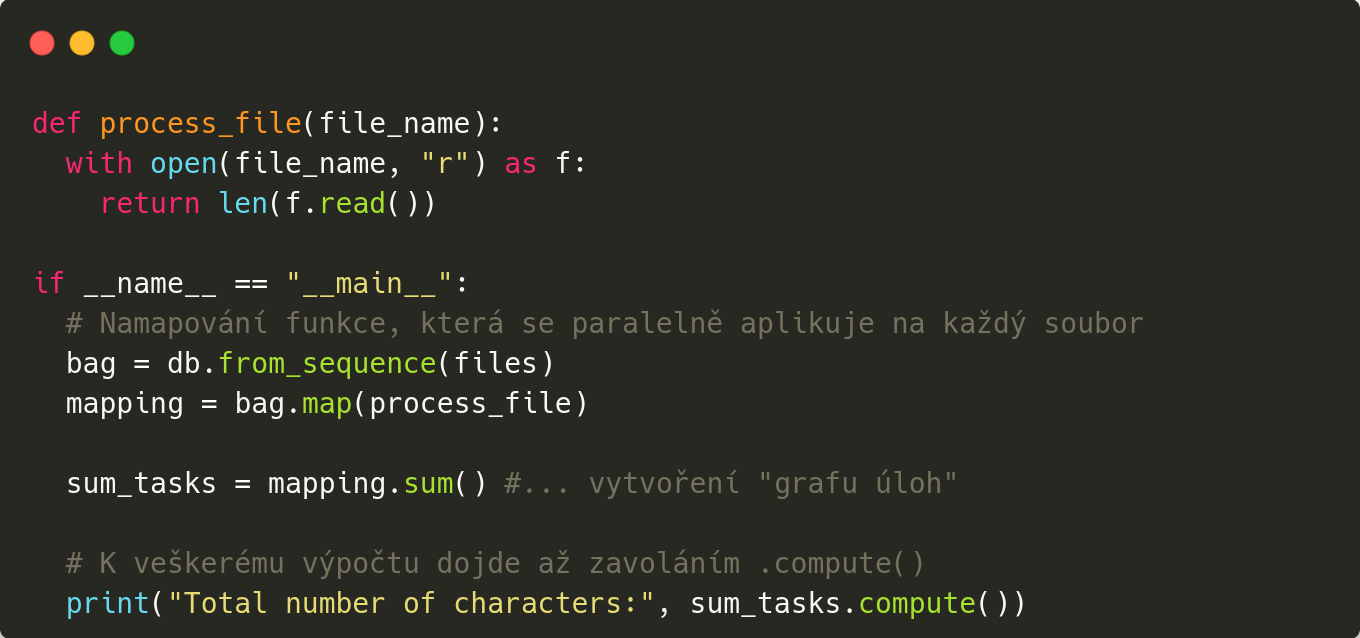
\includegraphics[width=\textwidth]{obrazky/codes/carbon15.png}
    \end{center}
\end{frame}



\begin{frame}{Odkládání výpočtu}
  % @dask.delayed
  % def inc(x):
  %    return x + 1

  % @dask.delayed
  % def add(x, y):
  %    return x + y
  
  % a = inc(1)       \# neprovede výpočet
  % b = inc(2)       \# neprovede výpočet
  % c = add(a, b)    \# neprovede výpočet
  
  % c = c.compute()  \# Vykoná všechny výpočty výše
    \begin{center}
        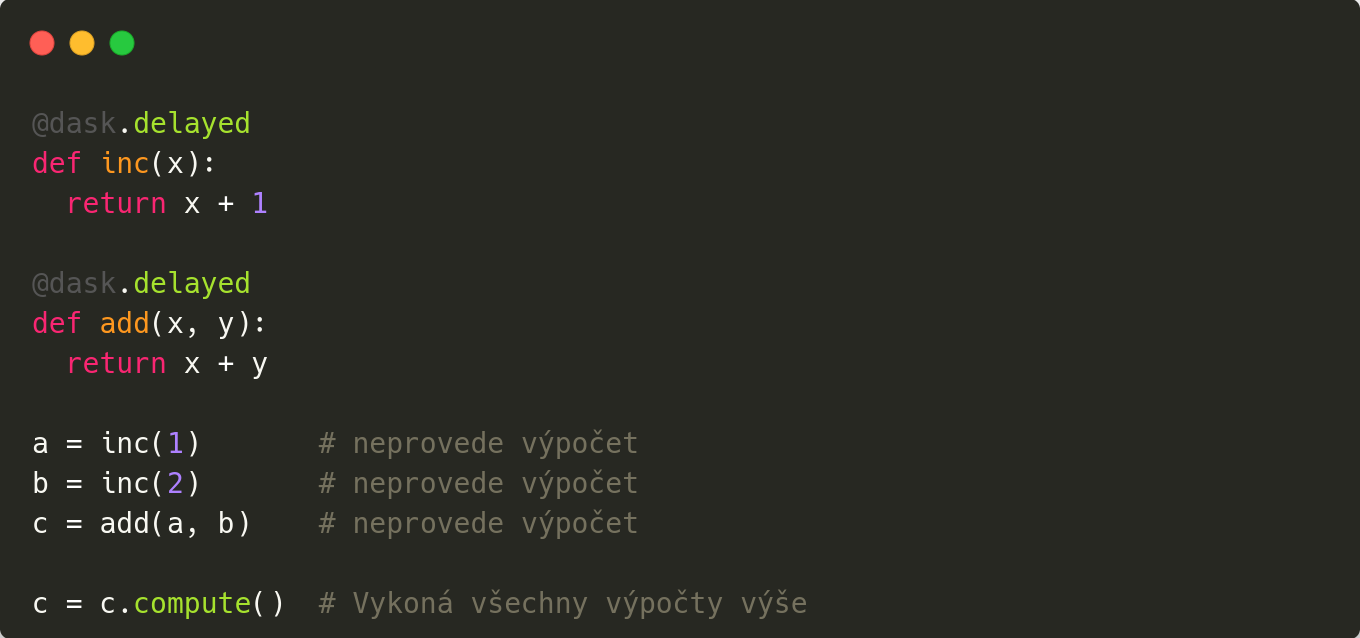
\includegraphics[width=\textwidth]{obrazky/codes/carbon16.png}
    \end{center}
\end{frame}

\section{Nástroje pro distribuované systémy}
\subsection{Knihovna socket}
\begin{frame}{Knihovna socket}
	\begin{itemize}
		\item Modul \texttt{socket} je základní nástroj pro implementaci síťové komunikace.
		\item Je \textbf{nízkoúrovňový} – jsou na něm založeny všechny ostatní moduly Pythonu vyšší úrovně pro propojení v síti.
		\item Podporuje většinu běžných protokolů, včetně TCP a UDP.
		\item \textbf{Výhody:}
		\begin{itemize}
			\item Přímá kontrola nad socketovou komunikací.
			\item Flexibilita pro implementaci vlastních protokolů.
		\end{itemize}
		\item \textbf{Nevýhody:}
		\begin{itemize}
			\item Vyžaduje znalosti síťových protokolů.
			\item Implementace složitější logiky (např. HTTPS) je náročnější.
		\end{itemize}
	\end{itemize}
\end{frame}

\begin{frame}{Knihovna socket - tvorba socketu}
    % import socket
    % 
    % socket = socket.socket(
    % 	family=AF\_INET,
    % 	type=SOCK\_STREAM
    % )
    \begin{center}
        
\includegraphics[width=\textwidth]{obrazky/codes/carbon10.png}
    \end{center}
	\begin{itemize}
		\item \texttt{family}  - určuje, jaký protokol se použije na síťové vrstvě.
		\begin{itemize}
			\item \texttt{socket.AF\_INET} - pro IPv4 adresy.
			\item \texttt{socket.AF\_INET6} - pro IPv6 adresy.
			\item \texttt{socket.AF\_UNIX} - Unixový socket (pro lokální komunikaci mezi procesy).
		\end{itemize}
		\item \texttt{type} - určuje, jaký protokol se použije na transportní vrstvě.
		\begin{itemize}
			\item \texttt{socket.SOCK\_STREAM} - používá TCP protokol.
			\item \texttt{socket.SOCK\_DGRAM} - používá UDP protokol.
		\end{itemize}
	\end{itemize}
\end{frame}

\begin{frame}{Knihovna socket - odeslání zprávy}
	% s.connect(('localhost', 12345)) \# navázání spojení
	% s.sendall(b'Ahoj!') \# odešle všechna data
	% s.close() \# ukončí socket s
    \begin{center}
        
\includegraphics[width=\textwidth]{obrazky/codes/carbon11.png}
    \end{center}
\end{frame}

\begin{frame}{Knihovna socket - poslouchání  a přijímání dat}
	% addr = ('localhost', 12345) \# adresa na které posloucháme
	% s.bind(addr) \# přiřadí socket k adrese
	% s.listen() \# umožňuje přijímat příchozí připojení
	% conn, addr = s.accept() \# čeká se na příchozí připojení
	% print(f'Připojeno: {addr}')
	% data = conn.recv(1024) \# přijme data, max. 1024B
	% conn.sendall(b'Ahoj!') \# pošle odpověď
	% conn.close() \# ukončí socket conn
	% s.close() \# ukončí socket s
    \begin{center}
        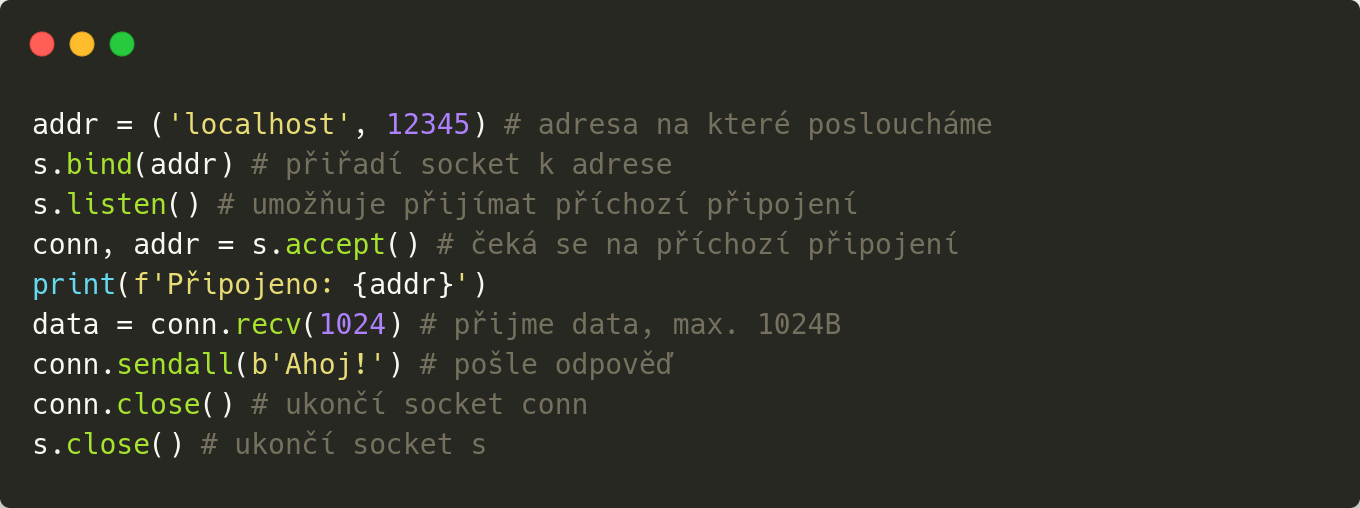
\includegraphics[width=\textwidth]{obrazky/codes/carbon12.png}
    \end{center}
\end{frame}

\subsection{Knihovna http.server}
\begin{frame}{Knihovna http}
	\begin{itemize}
		\item Modul \texttt{http} v Pythonu poskytuje nástroje pro práci s protokolem HTTP.
		\item Je rozdělen na několik podmodulů:
		\begin{itemize}
			\item Mezi ně patří např.: \texttt{http.client}, \texttt{http.server}, \texttt{http.cookies} \ldots
		\end{itemize}
		\item Využívá ho mnoho vyšších knihoven, jako je \texttt{requests} nebo \texttt{flask}.
		\item \textbf{Výhody:}
		\begin{itemize}
			\item Vyšší úroveň abstrakce.
			\item Snazší implementace běžných HTTP funkcionalit.
		\end{itemize}
		\item \textbf{Nevýhody:}
		\begin{itemize}
			\item Omezená flexibilita ve srovnání s nízkoúrovňovou komunikací pomocí \texttt{socket}.
		\end{itemize}
	\end{itemize}	
\end{frame}
\begin{frame}{Knihovna http.server}
	% from http.server import HTTPServer, BaseHTTPRequestHandler
    % 
	% class MyHandler(BaseHTTPRequestHandler):
    % 
	% 	 \# Definujeme metodu pro zpracování GET požadavků
	% 	def do\_GET(self):
	% 		pass
    % 
	% server = HTTPServer(("localhost", 8000), MyHandler)
	% print("Server bezi na portu 8000...")
	% server.serve\_forever()
    \begin{center}
        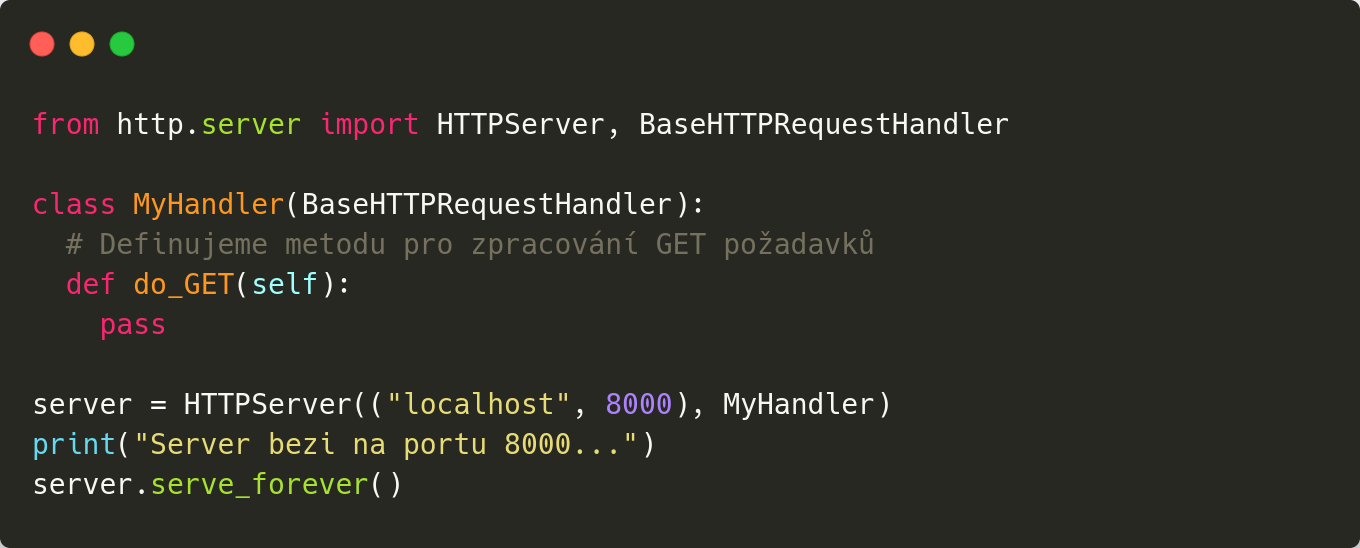
\includegraphics[width=\textwidth]{obrazky/codes/carbon13.png}
    \end{center}

	\begin{itemize}
		\item Dva typy serverů:
		\begin{itemize}
			\item \texttt{http.server.HTTPServer(args)}.
			\item \texttt{http.server.ThreadingHTTPServer(args)}.
		\end{itemize}
		\item Argumenty \texttt{args}:
		\begin{itemize}
			\item \texttt{server\_address} - dvojice IP adresa, port.
			\item \texttt{RequestHandlerClass} - zpracovává příchozí HTTP požadavky (např. GET, POST) a definuje, jak server na tyto požadavky odpoví.
		\end{itemize}
	\end{itemize}	
\end{frame}

\begin{frame}{Knihovna http.server}
	% def do\_GET(self):
	% 	\# Odeslání odpovědi s kódem 200 (OK)
	% 	self.send\_response(200)
	% 	\# Nastavení hlavičky Content-Type pro HTML obsah
	% 	self.send\_header("Content-type", "text/html") 
	% 	self.end\_headers()
	% 	\# Odeslání těla odpovědi – text "Hello, World!"     
	% 	self.wfile.write(b"Hello, World!")
    \begin{center}
        
\includegraphics[width=\textwidth]{obrazky/codes/carbon14.png}
    \end{center}
\end{frame}

\subsection{RabbitMQ}
\begin{frame}{RabbitMQ}
	\begin{itemize}
		\item Message broker implementující AMQP protokol.
		\item Usnadňuje komunikaci mezi aplikacemi nebo jejich částmi.
		\item Řeší problém výměny zpráv mezi producenty a konzumenty:
		\begin{itemize}
			\item [\textendash] Implementuje systém front zpráv.
			\item [\textendash] Exchanges (výměníky) jsou kompononenty zodpovědné za směrování zpráv 					  do správných front.
		\end{itemize}
	\end{itemize}

\end{frame}

\begin{frame}{Výhody RabbitMQ}
	\begin{itemize}
		\item Mezi hlavní výhody patří:
			\begin{itemize}
				\item [\textendash] Producenti nemusí čekat na zpracování zpráv (decoupling).
				\item [\textendash] Broker umožní jednodušší přidávání producentů nebo											  konzumentů (škálování).
				\item [\textendash] Samotný broker může pracovat na samostatném zařízení (výkon).
			\end{itemize}
	\end{itemize}
\end{frame}

\begin{frame}{Typy výměníků}
	\begin{columns}
    % Left column for bullet points
    \begin{column}{0.2\textwidth}
      \begin{itemize}
        \item Fanout
        \item Direct
        \item Topic
        \item Header
      \end{itemize}
    \end{column}
    
    % Right column for image
    \begin{column}{0.8\textwidth}
      \centering
      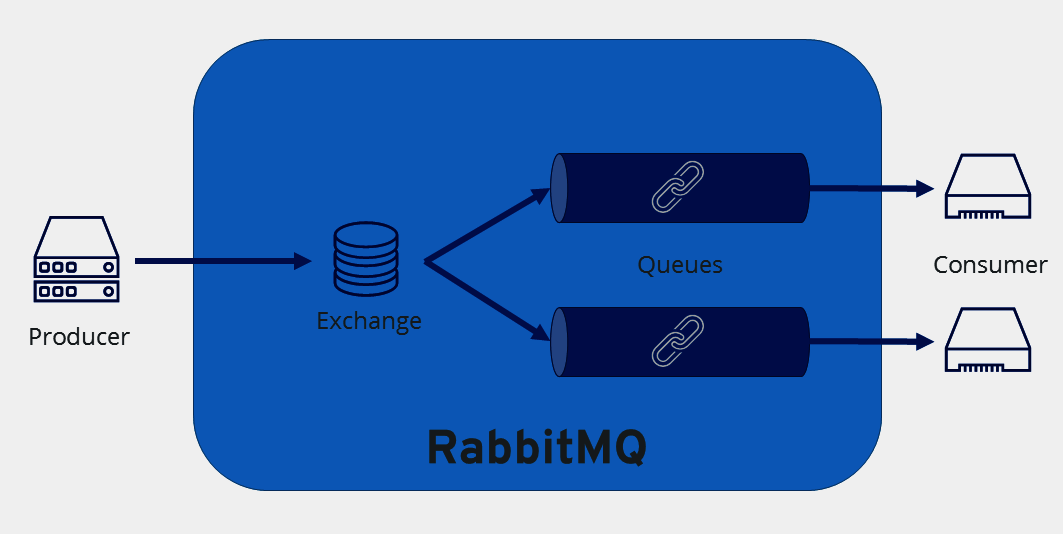
\includegraphics[width=\textwidth]{obrazky/rabbitmq.png}
    \end{column}
  \end{columns}
\end{frame}

\begin{frame}{Funkce a vlastnosti}
	\begin{itemize}
		\item Spolehlivost - zajištění neztracení zpráv.
		\item Flexibilita - Podpora různých protokolů (AMQP, MQTT, STOMP...).
		\item Škálovatelnost - jednoduchost rozšíření objemu zpracovávaných zpráv.
		\item Pluggability - jednoduchost rozšíření funkcionality.
	\end{itemize}
\end{frame}

\begin{frame}{Použití RabbitMQ}
	\begin{itemize}
		\item Asynchronní zpracování úloh
		\begin{itemize}
			\item [\textendash] Decoupling umožňuje zpracování úloh asynchronně bez nutnosti blokování producenta.
		\end{itemize}
		\item Load balancing
		\begin{itemize}
			\item [\textendash] Rozložení zátěže mezi více konzumenty.
		\end{itemize}
		\item Zpracování dat v reálném čase
		\begin{itemize}
			\item [\textendash] Monitoring, logování...
		\end{itemize}
		\item Příklady použití: Instagram, Reddit, SoundCloud...
	\end{itemize}
\end{frame}

\end{document}